%&pdflatex
\documentclass[12pt, twocolumn]{article}
\usepackage{caption}
\usepackage{chemformula}
\usepackage{enumitem}
\usepackage[outdir=../figures/]{epstopdf}
\usepackage{float}
\usepackage{fullpage}
\usepackage{graphicx}
\usepackage{hyperref}
\usepackage{microtype}
\usepackage{minted}
\usepackage{setspace}
\usepackage[caption=false]{subfig}
\usepackage{titlesec}

% \newcommand\TestAppExists[3]{#2}

\captionsetup{font=footnotesize}

\hbadness=99999  % or any number >=10000

\graphicspath{{../figures/}}

\titleformat{\section}{\normalfont\scshape}{\thesection}{1em}{}
\titleformat{\subsubsection}{\normalfont\scshape}{\thesection}{1em}{}

\newcommand*{\nolink}[1]{%
\begin{NoHyper}#1\end{NoHyper}%
}


\begin{document}

\title{Molecular Dynamics Simulation of the D102A Variant of Chymotrypsin}
\author{David Li, Patrick Fleming}
\date{\today}
\maketitle

\section{Introduction}
Almost one third of all proteases can be classified as serine proteases
~\nolink{\cite{hedstrom02}}. These proteins are named for the nucleophilic Ser
residue at the active site. Serine proteases fall into two broad categories
based on their structure: chymotrypsin-like (trypsin-like) or subtilisin-like
~\nolink{\cite{madala10}}. Chymotrypsin-like proteases are the most abundant in
nature and can be found in eukaryotes, prokaryotes, archae, and viruses. They
are involved in many critical physiological processes, such as hemostasis,
apoptosis, digestion, and reproduction~\nolink{\cite{hedstrom02}}.

In order to hydrolyze a peptide bond, these well-studied enzymes must overcome
three major mechanistic barriers: (i) amide bonds are extremely stable due to
electron donation from the amide nitrogen to the carbonyl; (ii) water is a poor
nucleophile and proteases always activate water via a general base; (iii) and
amines are poor leaving groups because proteases protonate the amine prior to
expulsion~\nolink{\cite{hedstrom02}}.

To overcome these three reaction barriers, serine proteases contain a group
of three residues called the catalytic triad that use hydrogen bonding to
increase reaction favorability. In chymotrypsin, the triad is composed of
serine, histidine, and aspartate, and is part of a larger hydrogen bonding
network~\nolink{\cite{hedstrom02}}.

\begin{figure}[H]
    \subfloat[Wild-Type\label{fig:triad_wt}]{
        \frame{
            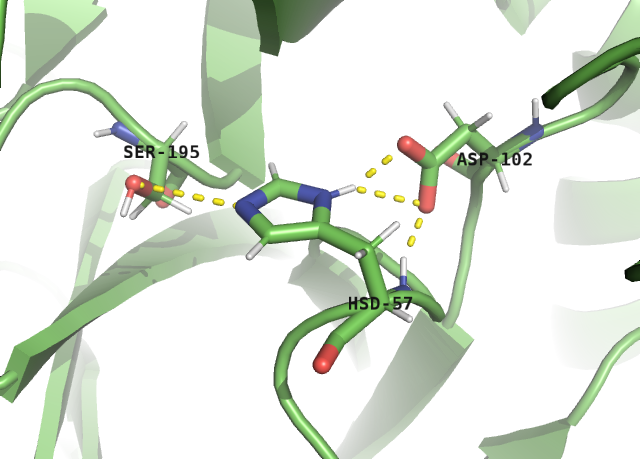
\includegraphics[trim={0 0 0 1}, clip, width=0.45\textwidth]
                {wt_conformation1.png}
        }
    }

    \subfloat[D102A variant\label{fig:triad_d102a}]{
        \frame{
            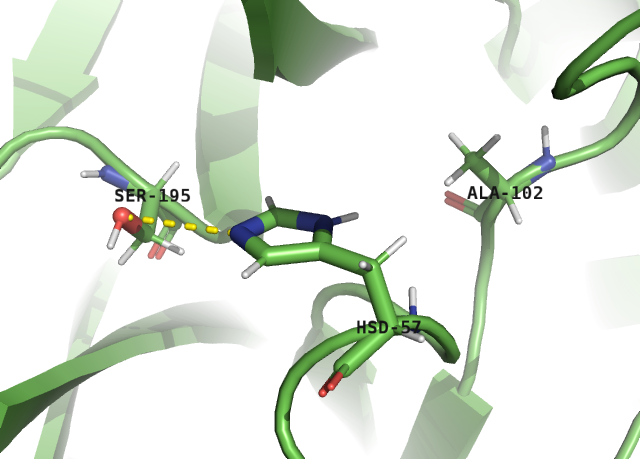
\includegraphics[trim={0 0 0 1}, clip, width=0.45\textwidth]
                {d102a_conformation1.png}
        }
    }
    \caption{Conformation of catalytic triad structure in wild-type and D102A
    variant of chymotrypsin}\label{fig:triad}
\end{figure}

Mutagenesis experiments of catalytic
triad residues show decreased catalytic activity; substitution of Ser195 or
His57 with Ala effectively disables the triad~\nolink{\cite{hedstrom02}}. For
this project, we hypothesize that the Asp-His hydrogen bond restrains the
conformational flexibility of the His ring so that it can more strongly
hydrogen bond to Ser, thus activating serine for a nucleophilic attack.

To test this, we carried out two all-atom molecular dynamics simulations of
two chymotrypsin series variants: the wild type sequence, and with Asp-102
substituted for alanine (mutation D102A). This enabled us to determine rotamer
distributions of the His side chain and the time-dependent frequencies of
His-Ser bond formations.

\section{Methods}

A chymotrypsin from \textit{Bos taurus}
(RCSB PDB ID:\@ \href{http://www.rcsb.org/pdb/explore.do?structureId=1ggd}{1GGD})
was used as the starting structure, with an additional calcium atom added to
stabilize the enzyme. The charged form of aspartate (ASP) and the neutral form
of histidine (HSD) were used when building the system with VMD 1.9.3. After
stabilizing, VMD was used to neutralize the system with water and 0.2M \ch{KCl}.
The D102A system was created using the same parameters, solvation, and
neutralization as the wild-type system but the catalytic triad aspartate was
mutated to an alanine residue.

After these steps, the wild-type system contained 16142 atoms and the D102A
system contained 16138 atoms. Both systems were centered about the origin and
the B-factor of the protein atoms was set to 1.00. The minimum and maximum
coordinates of the system were then calculated in order to set the bounding
box for periodic boundary conditions with side length of 60\AA{} in all 3
coordinate directions.

The systems were simulated in an isobaric ensemble (NPT conditions), with a
temperature of 298.15 K and pressure of 1 atmosphere. To control temperature,
Langevin dynamics were used with a coupling coefficient
\(\gamma = 1 \mathrm{ps}^{-1}\). To maintain constant pressure, a Langevin
piston Nos\'e-Hoover method was used in NAMD with a piston period of
100 fs and a piston decay of 50 fs~\nolink{cite{namd05}}. Finally, the CHARMM
force field was used to calculate interatomic forces with a cutoff distance
of 12\AA{}.

Both simulations were run through three equilibration runs and one production
run. The first equilibration run had a 1 fs time-step and was run for 10000
steps (10 ps simulation), and water molecules were free to move around the
fixed protein.
The second equilibration run had a 1 fs time-step and was run for 10000 steps
(10 ps simulation), but in this case both water and protein were free to move.
The third and final equilibration run had a 2 fs time-step and was run for
2500000 steps (5 ns simulation), and again, both water and protein were free
to move.
The production run used a 2 fs time-step and was run for 5000000 steps (10 ns
simulation) with a frame capture every 2 ps for a total of 5000 frames in the
resulting dcd trajectory file.

Simulations were conducted on the JHU Biophysics kirin cluster running Ubuntu
12.04 with 12 computation nodes.

\section{Results}

Figure~\ref{fig:triad} shows the catalytic triads of the wild-type and mutated
chymotrypsin. Comparing figure~\ref{fig:triad_wt} and
figure~\ref{fig:triad_d102a} shows the loss of three Asp-His hydrogen bonds
in the mutant. These hydrogen bonds are the ones that we hypothesized to
conformationally restrain the histidine.

The root-mean-square deviation (RMSD) of atomic positions of the D102A variant
was determined to be slightly higher than
that of the wild-type variant, with an average of 2.09\AA{} compared to
2.00\AA{}. As seen in Figure~\ref{fig:rmsd}, after about 8 ns of simulation,
the D102A RMSD sharply increases to around 2.5\AA{}, indicative of a loop
flexing out, which can be confirmed from visual inspection of the trajectory.


\begin{figure}[H]
    \centering
        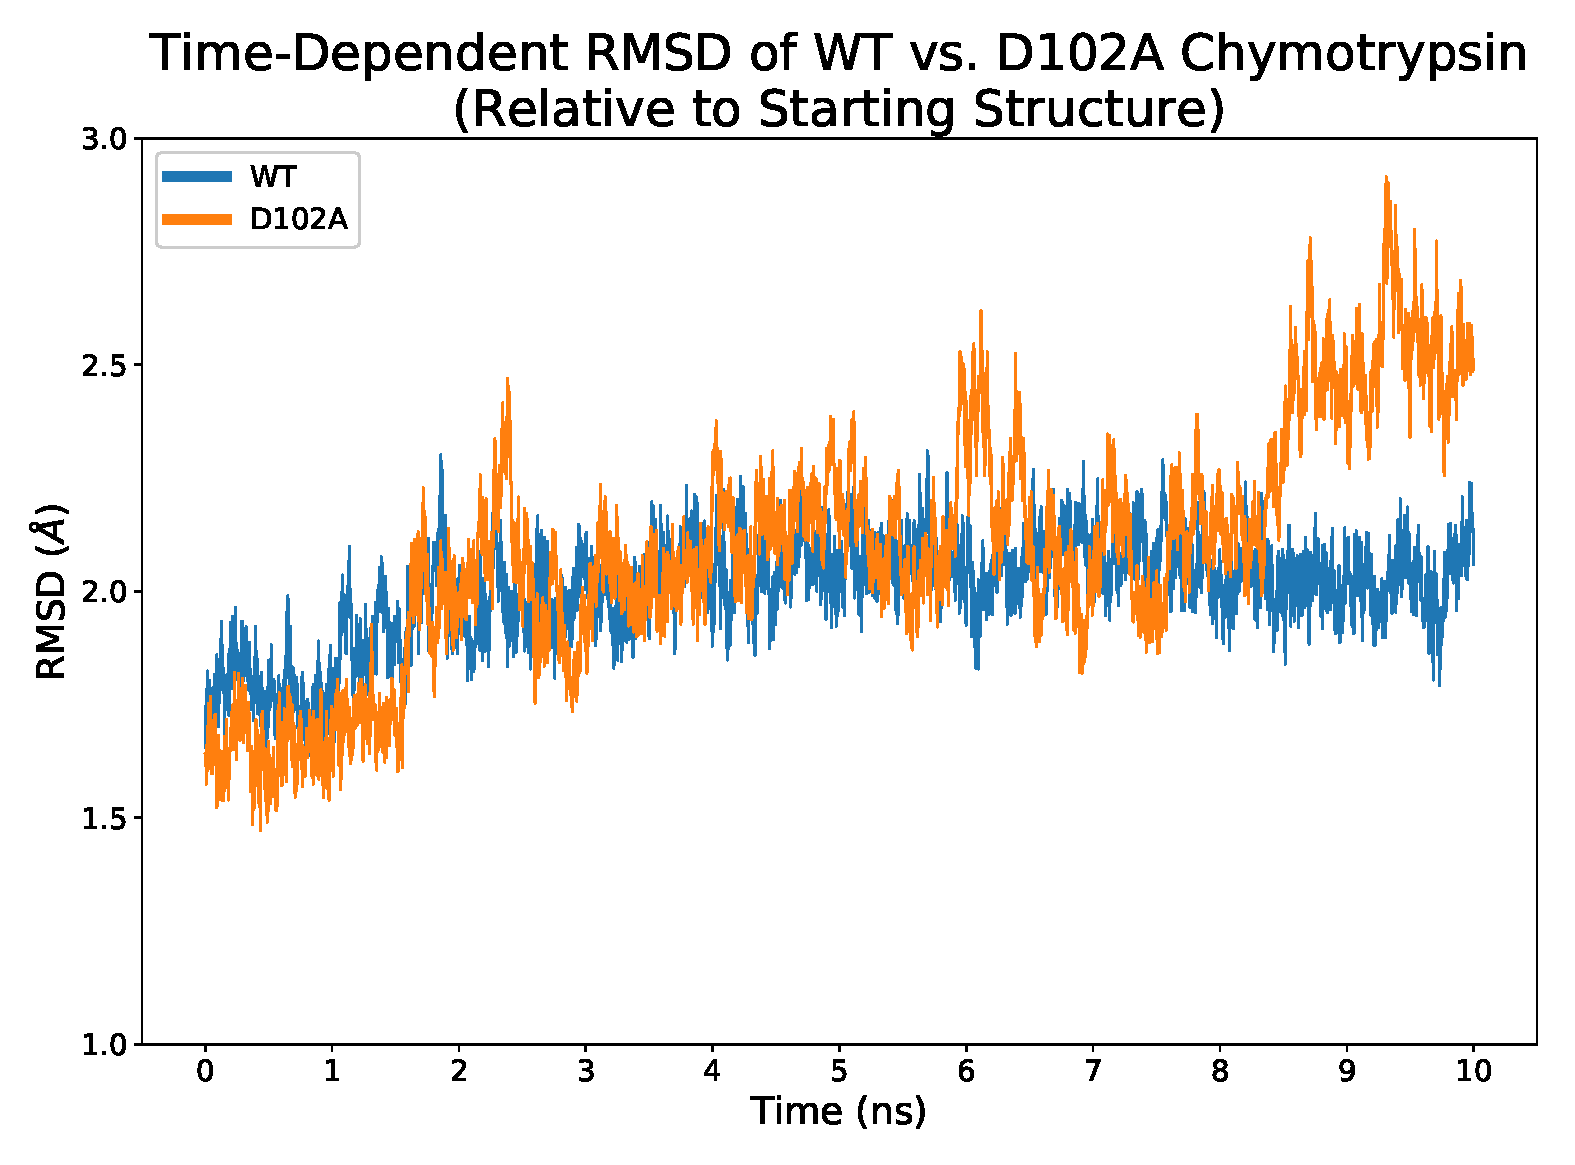
\includegraphics[width=0.49\textwidth]{rmsds.eps}
    \caption{RMSD of wild-type (WT) and D102A simulations}\label{fig:rmsd}
\end{figure}

\begin{figure}[H]
    \centering
        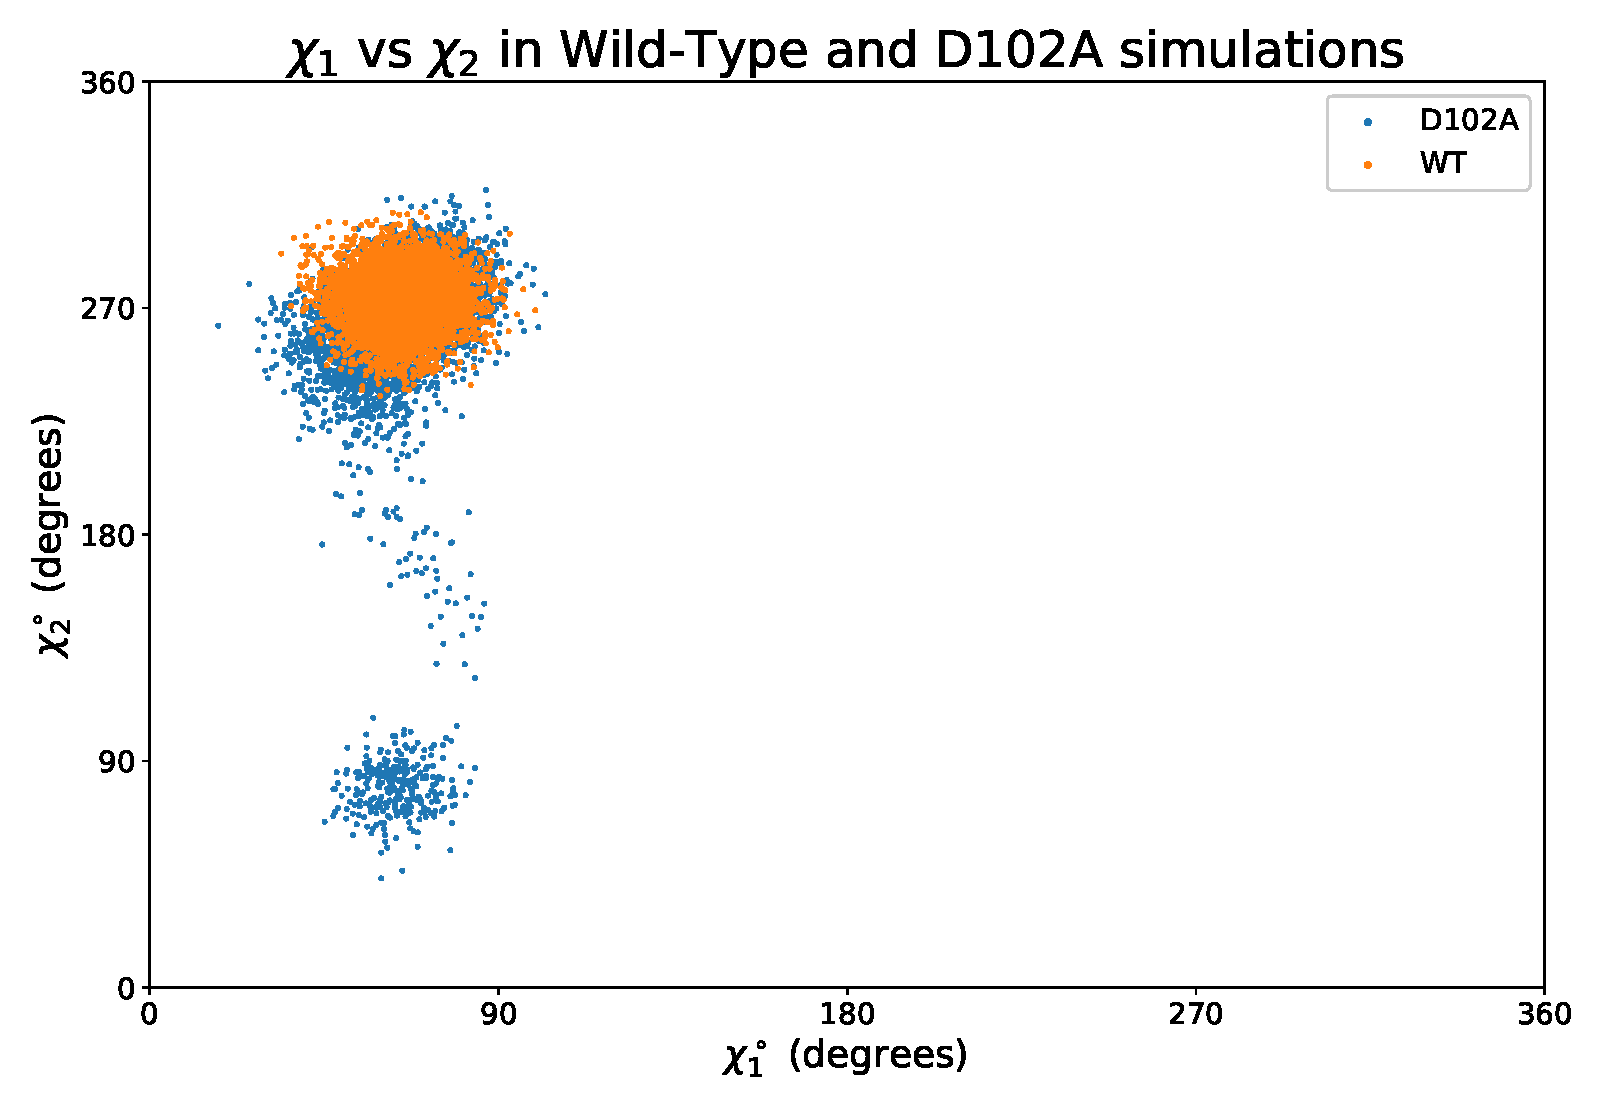
\includegraphics[width=0.49\textwidth]{chi_plot_wt_d102a.eps}
    \caption{Dihedral bond angle distribution for Histidine Side Chains
        in wild-type and D102A simulations}\label{fig:chiplot}
\end{figure}

The dihedral angle between H59 \(\alpha\)-carbon and \(\beta\)-carbon
(\(\chi_1\)) and the dihedral angle between H59 \(\beta\)-carbon and
\(\gamma\)-carbon (\(\chi_2\)) were measured for each frame in the WT and
D102A simulations. As seen in Figure~\ref{fig:chiplot}, the D102A variant
showed significantly higher variability in dihedral angles, where the
distribution appeared to be bimodal with two peaks at
\(\chi_2 \approx 90^\circ\) and \(\chi_2 \approx 270^\circ\). In
the region with \(\chi_2 \approx 270^\circ\), the mutant sampled a wider
range of bond angles.


\begin{figure}[H]
    \centering
        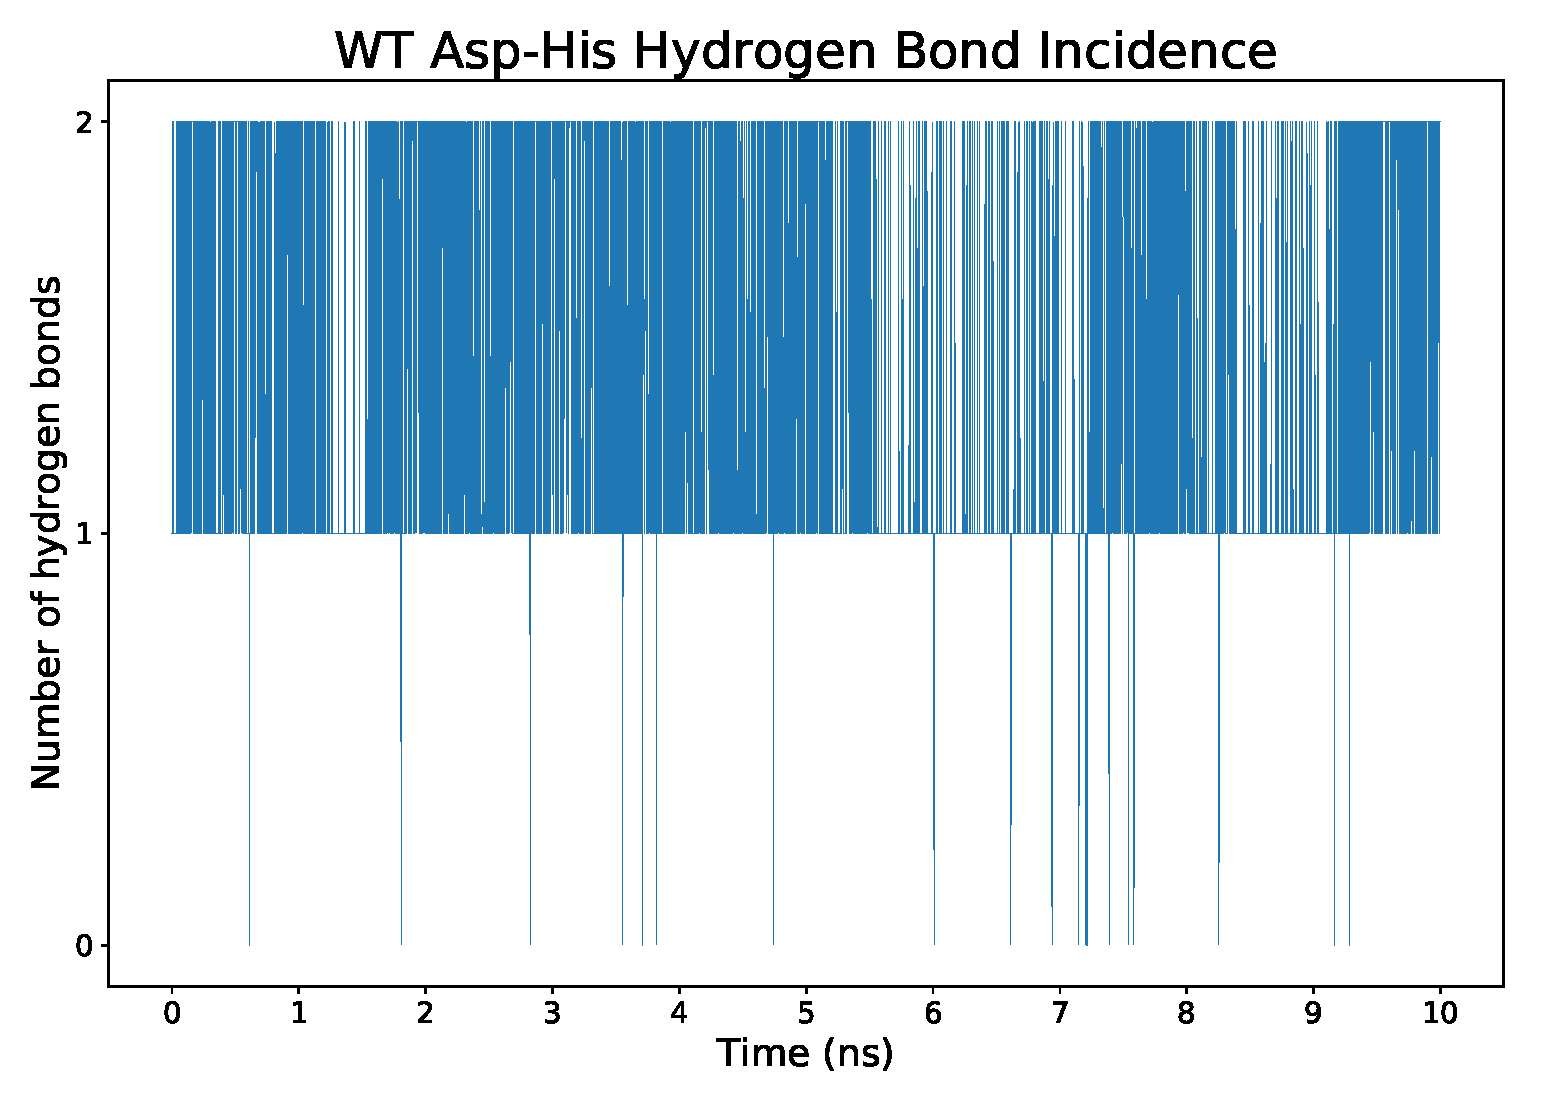
\includegraphics[width=0.49\textwidth]{wt_hbonds_asp_his.eps}
    \caption{Rapid Conversion between 1 and 2 Asp-His hydrogen bonds
        of wild-type chymotrypsin indicates persistent bond}
\end{figure}


\begin{figure}[H]
    \centering
        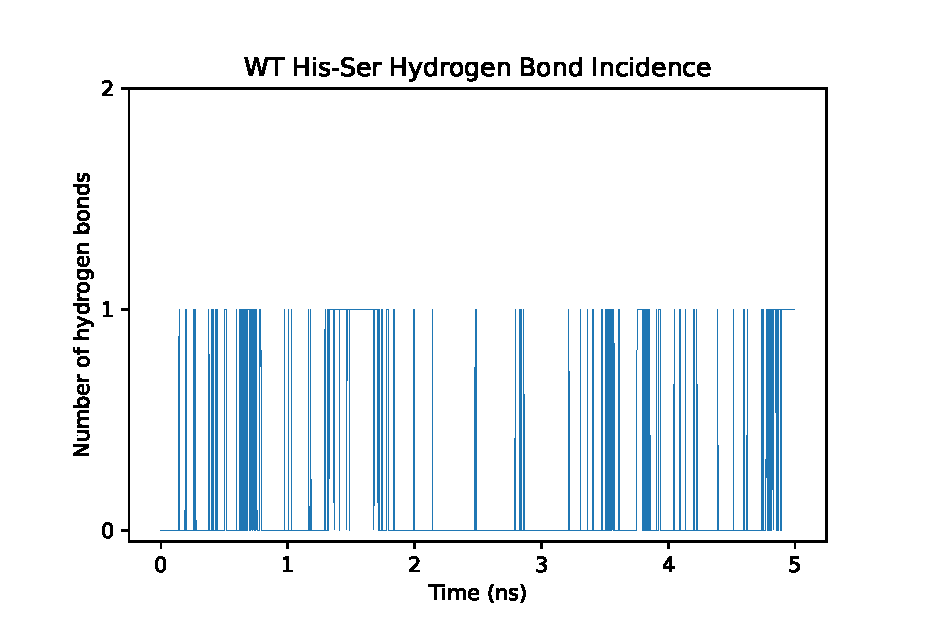
\includegraphics[width=0.49\textwidth]{wt_hbonds_his_ser.eps}
    \caption{}
\end{figure}

\begin{figure}[H]
    \centering
        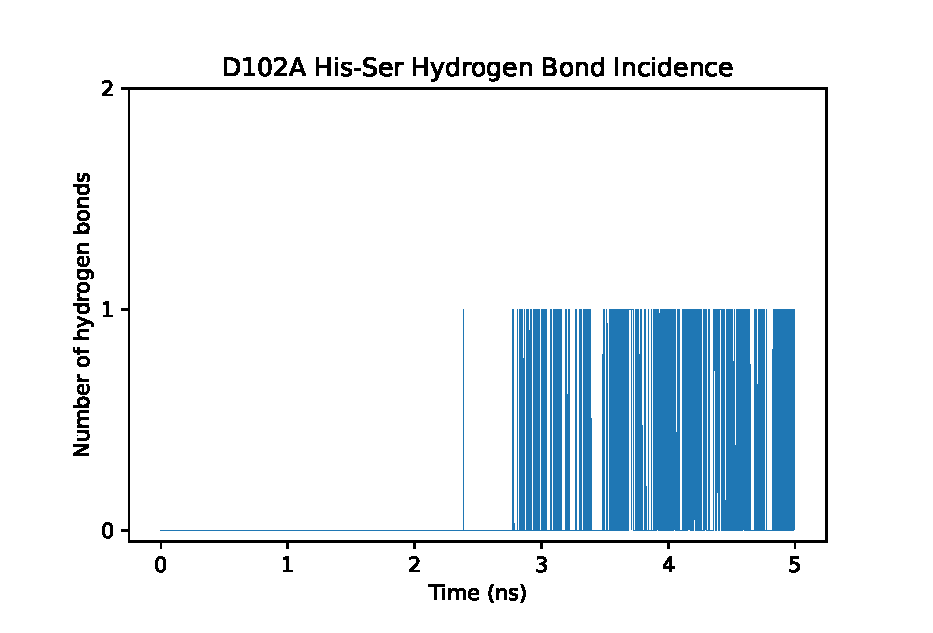
\includegraphics[width=0.49\textwidth]{d102a_hbonds_his_ser.eps}
    \caption{}
\end{figure}


\begin{figure}[H]
    \centering
    \subfloat[Wild Type\label{fig:lifetime_wt}]{
        % \frame{
            \centering
            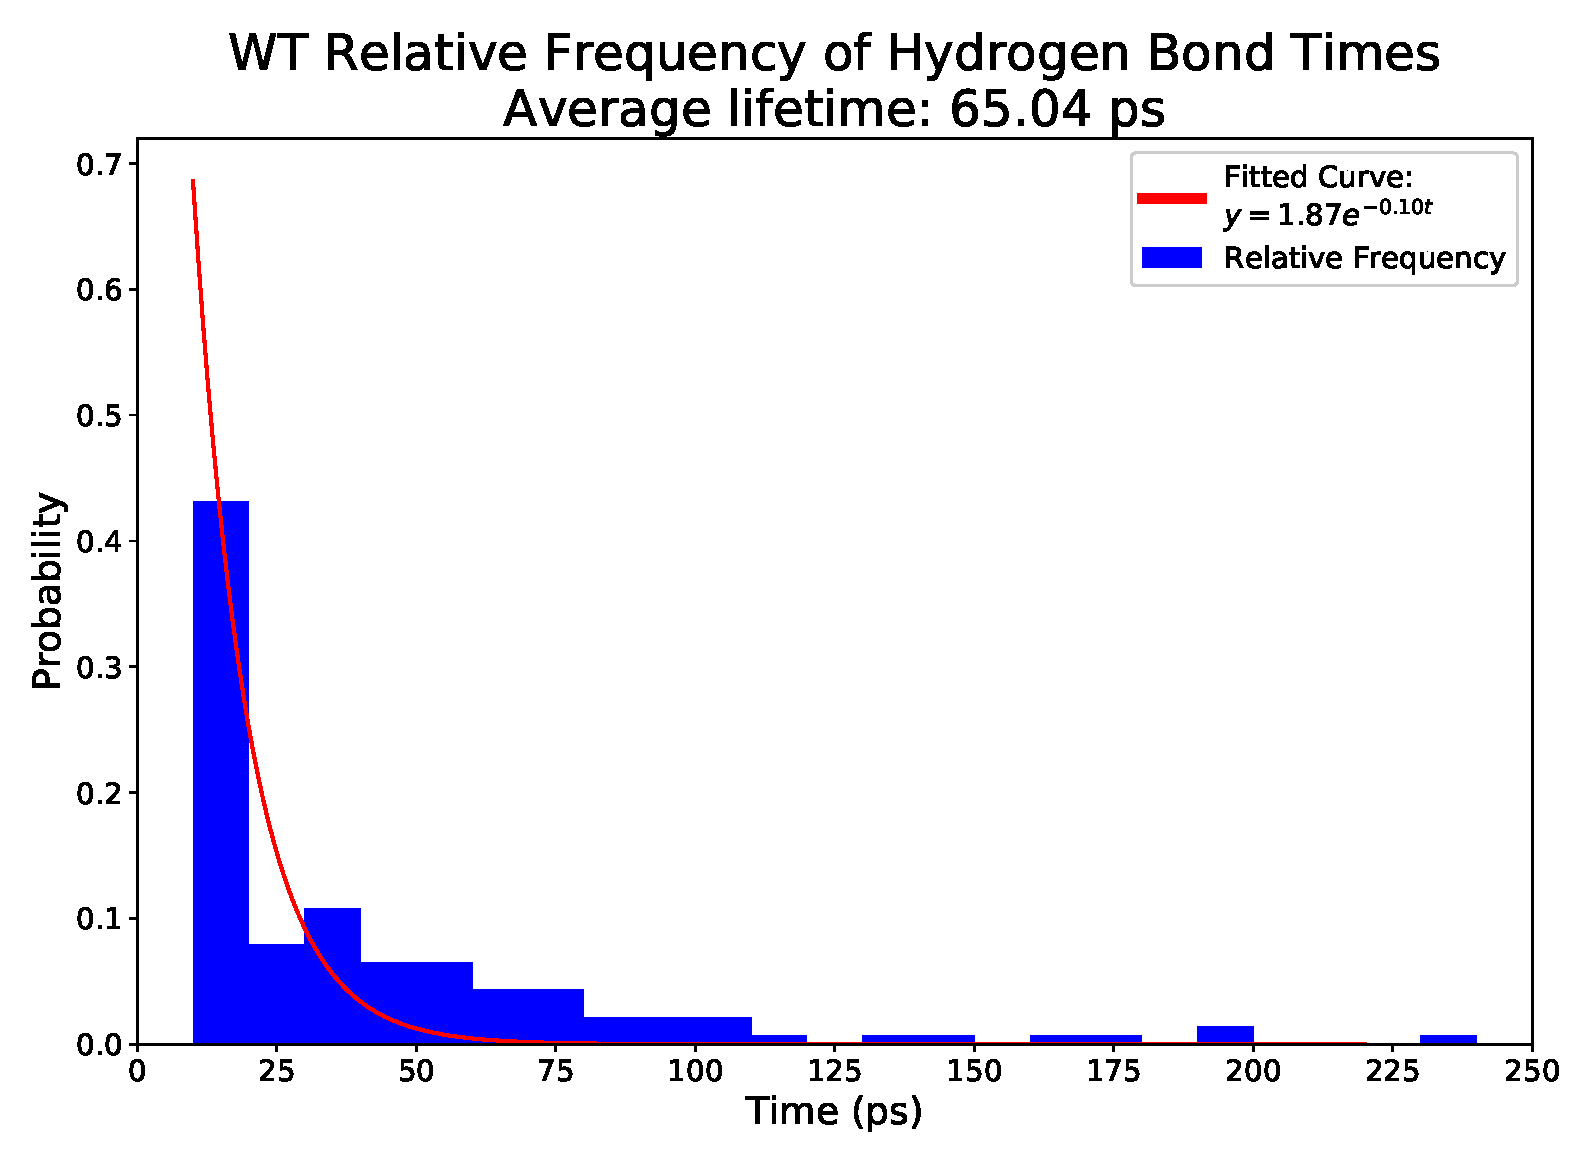
\includegraphics[width=0.49\textwidth]{wt_hbond_times.eps}
        % }
   }

    \subfloat[D102A\label{fig:lifetime_d102a}]{
        % \frame{
            \centering
            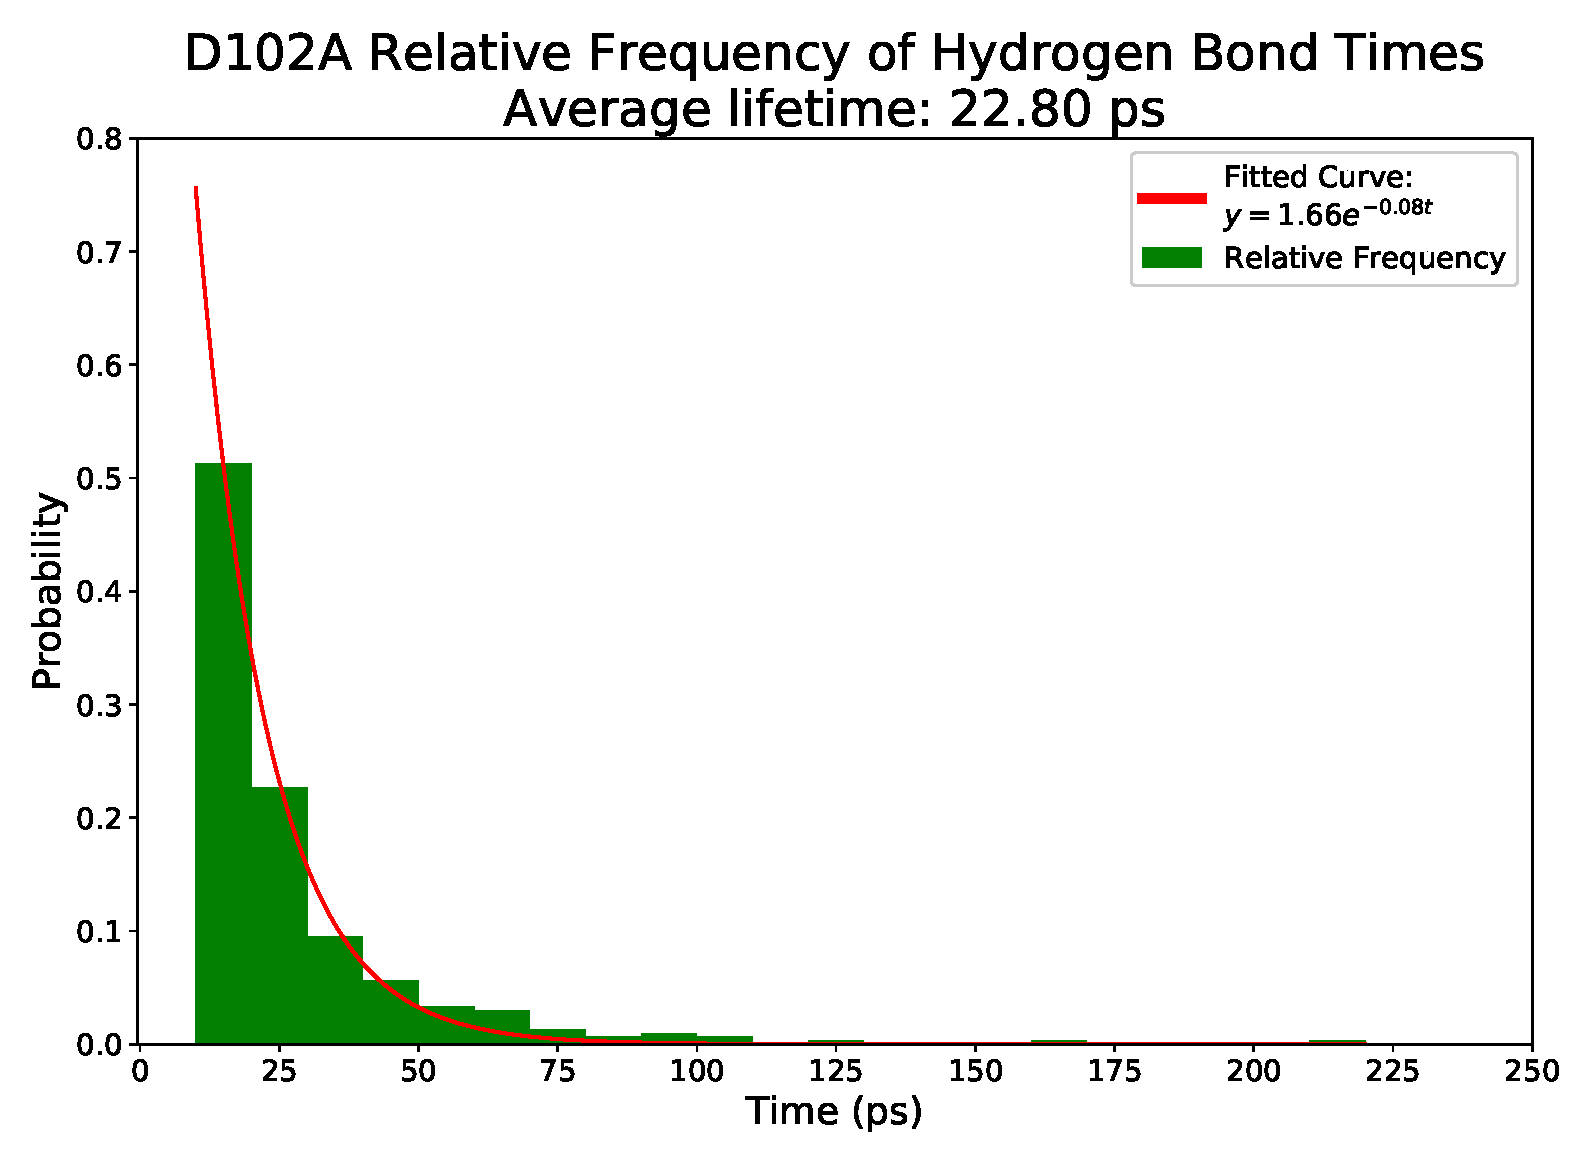
\includegraphics[width=0.49\textwidth]{d102a_hbond_times.eps}
        % }
    }

    \caption{}
\end{figure}


\section{Conclusion}

\subsubsection*{Acknowledgements}

\section{References}
\begin{thebibliography}{9}
\bibitem{hedstrom02}
Hedstrom L. Serine protease mechanism and specificity.
Chemical reviews. 2002 Dec 11; 102(12):4501--24.

\bibitem{madala10}
Madala PK, Tyndall JD, Nall T, Fairlie DP.\@
Update 1 of: Proteases universally recognize beta strands in their
active sites. Chemical reviews. 2011 Apr 8; 110(6):PR1--31.

\bibitem{namd05}
Phillips JC, Braun R, Wang W, Gumbart J, Tajkhorshid E, Villa E,
Chipot C, Skeel RD, Kale L, Schulten K. Scalable molecular dynamics
with NAMD.\@ Journal of computational chemistry. 2005 Dec 1;26(16):1781--802.

\end{thebibliography}

\appendix

\onecolumn
\begin{minted}{python}
    from matplotlib import pyplot as plt
    from __future__ import division
    from scipy.optimize import curve_fit
    import numpy as np

    """
    Hydrogen bonds involving last frame are intentionally omitted
    since their duration cannot be calculated
    """

    #prev tracks if hbond in previous frame
    #hbond is bond status
    #count is bond duration
    prev = hbond = count = 0
    sizes = [] #list of bond durations
    with open("../D102A/hbonds_his_ser.dat") as f:
        for line in f:
            line = line.split() #splits line by whitespace
            hbond = int(line[1])
            if hbond == 1:
                count += 1
                prev = 1
            elif hbond == 0 and prev == 1:
                #if the hbond terminates
                sizes.append(count)
                count = prev = 0
            else:
                #hbond == 0 and prev == 0, nothing happens
                continue

    sizes = [x*10 for x in sizes]
    #weighting for relative frequency
    weights = np.ones_like(sizes)/float(len(sizes))
    # print(sum(sizes)/len(sizes)) #prints average lifetime

    #Plotting & Saving
    plt.figure(figsize=(12, 8))
    #Histogram
    n, bins, patches = plt.hist(sizes, color='b', weights=weights,\
                bins=range(10, max(sizes)+20, 10), label='Relative Frequency')

    def func(x, a, b):
        return a * np.exp(-b * x)

    #Best-fit exponential
    bins = [0.5*(bins[i]+bins[i+1]) for i in range(len(bins)-1)]
    popt, pcov = curve_fit(func, bins, n, p0=(4, 0.1))
    x = np.linspace(10, 220, 2100)
    A, K = popt

    #Plot best-fit exponential
    plt.plot(x, func(x, *popt), 'r-',\
            label='Fitted Curve:\n$y = %0.2f e^{-%0.2f t}$' % (A, K))

    #Labeling
    plt.title("WT Relative Frequency of Hydrogen Bond Times\n\
            Average lifetime: {:0.2f} ps".format(sum(sizes)/len(sizes)), fontsize=24)
    plt.xlabel("Time (ps)", fontsize=18)
    plt.ylabel("Probability", fontsize=18)
    plt.xlim((0, 250))
    plt.xticks(np.arange(0, 251, 25), fontsize=14)
    plt.yticks(np.arange(0, 0.71, 0.1), fontsize=14)

    #legend formatting
    lgnd = plt.legend(prop={'size': 14})
    lgnd.legendHandles[0].set_linewidth(5.0)
    lgnd.legendHandles[1].set_linewidth(5.0)
    plt.savefig('../figures/wt_hbond_times.eps',\
            format='eps', dpi=1000, bbox_inches='tight')
\end{minted}

\end{document}